\documentclass{article}
\usepackage{graphicx}

\begin{document}

\title{Status Report \#0}
\author{Nicolà Lohr}

 \maketitle
\newpage
\begin{abstract}

Completed so far:
\begin{itemize}
\item Basic knowledge of \LaTeX
\item This Short Status Report
\item Decision on the scope and the time commitment: "KSZ great"
\item Book selection: Data Science from Scratch (9781491901427), Data Algorithms (9781491906187)
\end{itemize}
\end{abstract}
\section{Introduction}
The first proof of concept indicates that the original aims are achievable: I am able to link every MAC-address to a class or teacher at least. Finding close friends works as well. I also learnt the basics of \LaTeX.
\section{Details}
\subsection{\LaTeX}
I learnt the basic of \LaTeX for the final paper. I'm writing/wrote this report also in \LaTeX to improve my skills. 
\subsection{Time-Commitment}
Because of the limited time in the year of 2019 I chose to focus on making a great high school project and paper and not on making an "ETH great" paper.
\subsection{Books}
I selected the two books I am going to read over the summer holidays. I used Safari Books for evaluating as many books as possible to find the best for my needs. I choose Data Science from Scratch and Data Algorithms. Both of these books should give me more inside in useful algorithms for my next steps. The first book should also help to improve my coding skills. Data preprocessing and graphics are covered as well.
\subsection{Proof of Concept}
\subsubsection{Basic Tracking}
The basic tracking links the MAC address of the user to his or her class. First I parse the data from the time table into a dictionary so it is easy to extract the class and the teacher from the weekday, room and time. I stored all the log-files from the IT-department in one folder. Next step is to get all this data into a useful format. The program is using tuples with the format: (time, user-mac, ap-place). Afterwards, the program filters the data to get rid of the part of the data which have nothing to do with the target subject. With just the relevant data, it's just a comparison between the data and the parsed time-table and the program tries to find as many matches as possible. The class with the most matches will then be presented as a result.
\subsubsection{Reverse Tracking}
Reverse tracking is basically the tracking for all MAC addresses which are found in the log files. That the program doesn't have to run over a thousand times (for every MAC address once) I created the reverse tracking. The difference between the basic tracking and the reverse tracking is that reverse tracking isn't using a filter and goes therefore through all the data. As a result, the program returns a dictionary with all MAC-addresses and their potential class.
\subsubsection{Friends Tracking}
As a side project, I tried to find out who is friends with whom. I looked which people walked together so that their phones switched the access-point at about the same time (~5 sec). I mostly found friends who are in the same class (walk from one classroom to the next) but also had some success with students in different classes.
\subsubsection{Optimisation}
To optimise my program speed I parsed the data like mentioned in basic tracking, so I had to look at the files just once. I also used multiprocessing (running part of the program in parallel) to improve speed. Running multiple times the same program in the background came with not much gain of speed and the accuracy dropped a little. For the final version, I most likely won't have the multiprocessing as a standard. 
\subsection{Next Steps}
To be able to do more proof of concepts with different algorithms to find more interesting hidden information in the log-files, I'm going to read the selected books. Besides that, I'll start writing the paper and create a website for the public to raise more awareness. For the paper, I also need to research facts about the danger and misuse of metadata analysis.
\newpage
\section{Brainstorming}
Here is the brainstorming from one of the meetings with Wiwi:

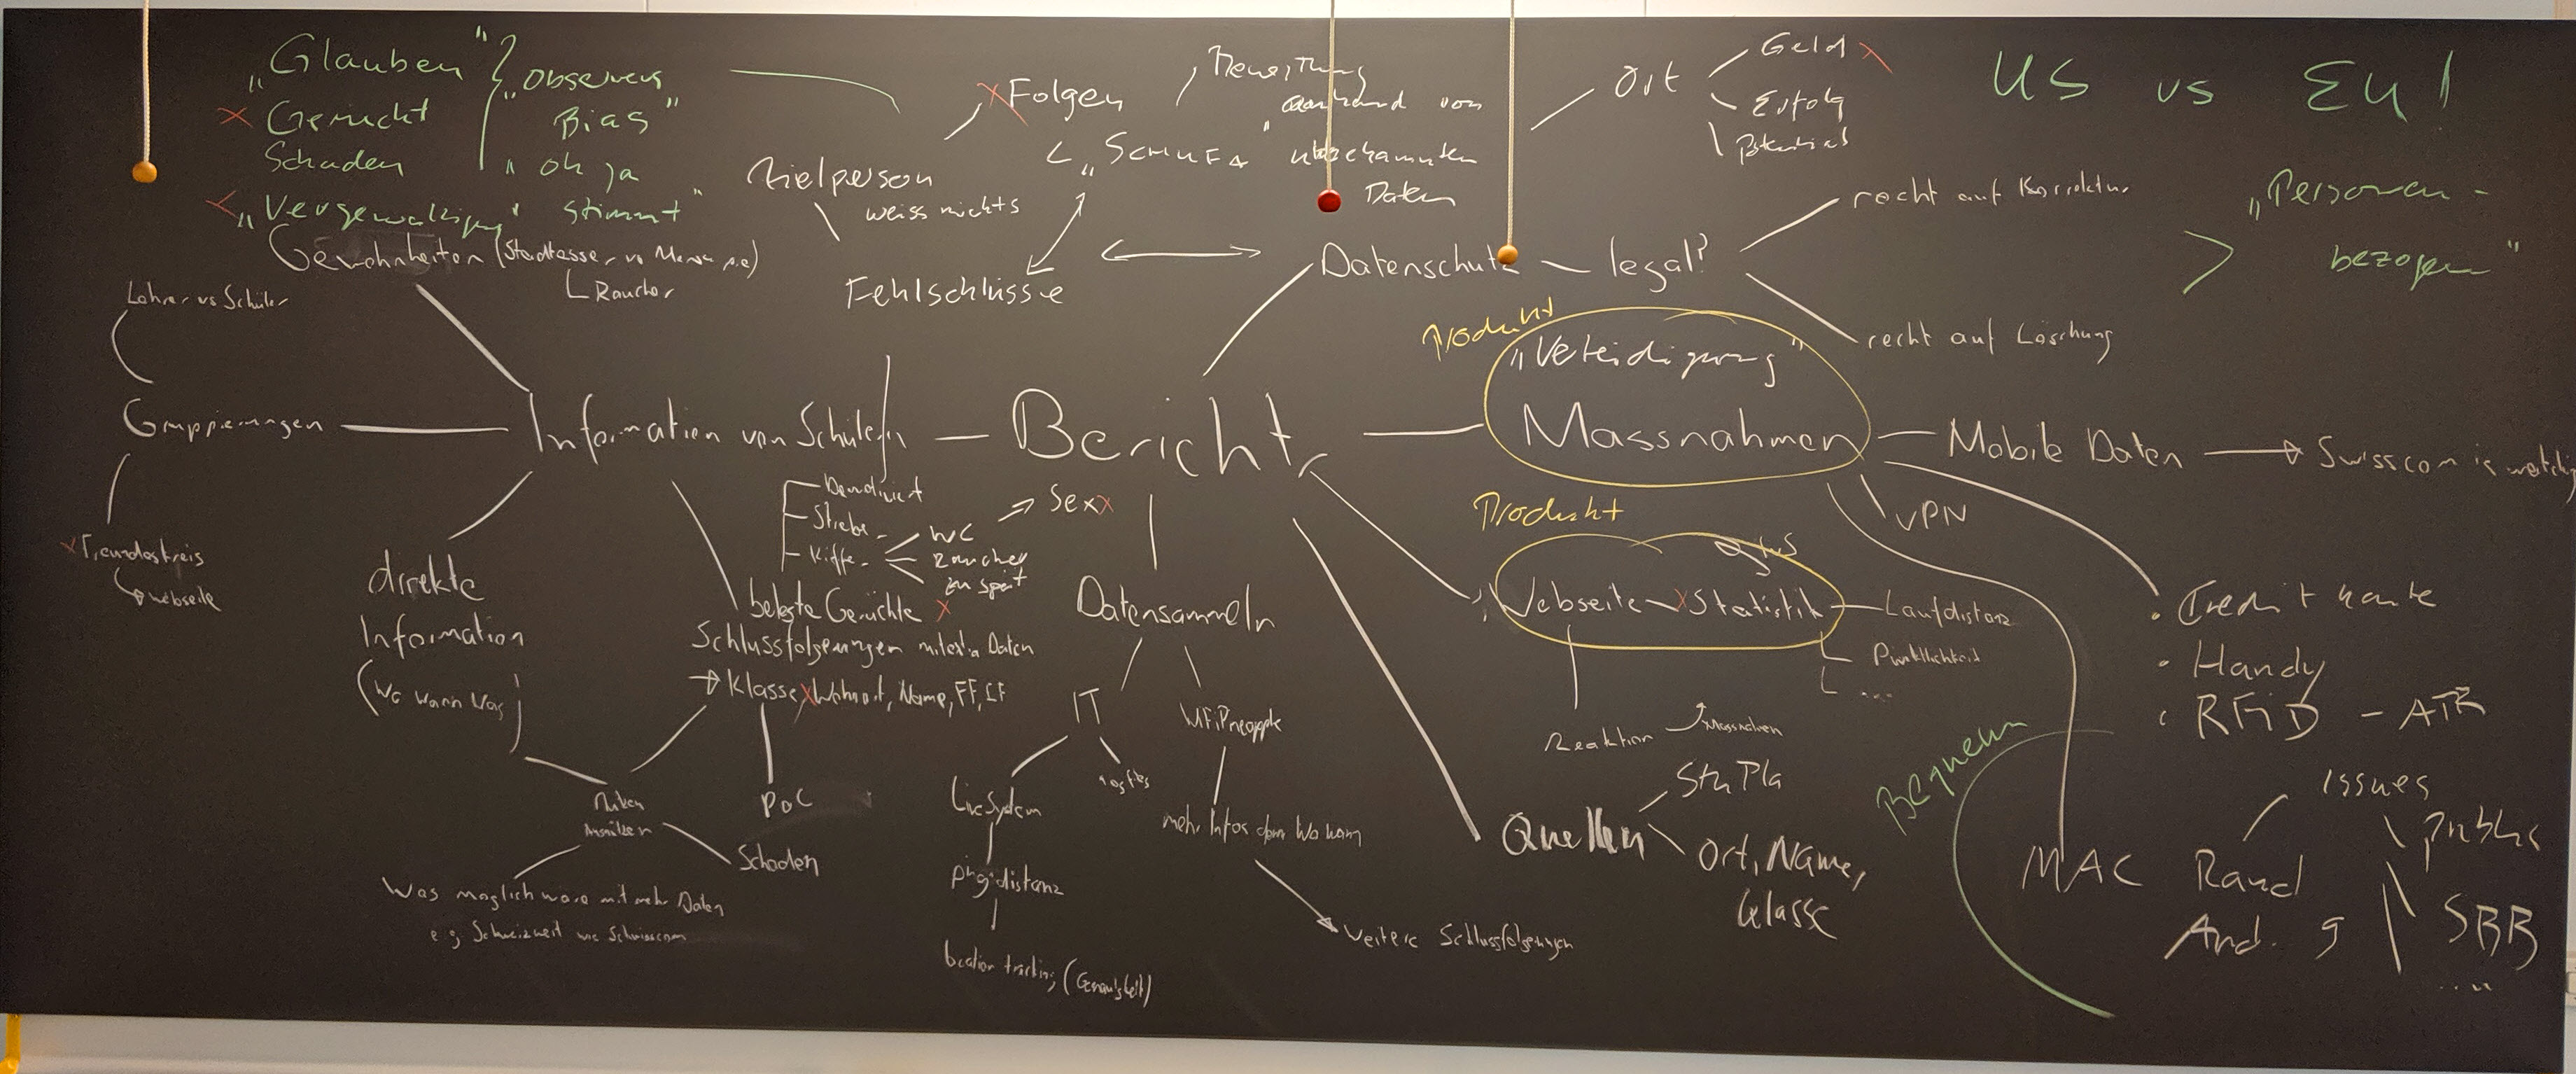
\includegraphics[width=\textwidth]{brainstorming}
 \end{document}
